\section{Experimental Evaluation}

We have implemented \compiler\ in OCaml and it is currently able to produce C++
code that may be compiled directly or embedded in another application. We now
experimentally evaluate the query executors produced by \compiler\ in a mix of
application scenarios. These include the order book application described in the
introduction, which to the best of our knowledge cannot be supported by existing
stream processing engines, nor do they execute efficiently on traditional
databases, as well as a subset of the Linear Road stream processing benchmark
that simulates a toll-charging system on a highway, and lastly an end-to-end
warehouse loading and analysis based on generating a star schema from a TPC-H
dataset and computing aggregations on the star schema.

\subsection{Experimental Setup}
We experimentally evaluated \compiler\ on Dual Intel Xeon 5335 processor (8
cores, 2.0Ghz), 16Gb RAM, running Red Hat Enterprise Linux 4 (Linux Kernel
2.6.18). Note that \compiler\ does not yet produce query executors capable of
exploiting multicore processing, thus our results represent query performance on
a single core. Following the generation of C++ code, we used \texttt{g++} v4.3.2,
compiling with optimization level '-O3', and additional optimization parameters
for aggressive inlining and loop optimizations.

\textbf{Data and query workloads.}
We discussed automated trading based on order book data in the introduction,
and use the VWAP query as one workload. The dataset feeding this query is the
TotalView-ITCH [XXX] historical order book from the NASDAQ stock exchange for a
3-month period from December 2008 to February 2009, for the MSFT (Microsoft)
symbol. This application captures the need for standing queries on temporal
snapshots which may be arbitrarily modified with inserts, deletes and updates,
and where the application is self-governing in ensuring order books do not grow
unboundedly.

The second workload we consider is a stream processing workload,
namely a subset of the Linear Road benchmark [XXX] responsible for detecting
accidents and assessing tolls on the highway. We are currently implementing the
full benchmark as part of ongoing work, and are expecting further
result improvements based on \compiler's ability to directly maintain
aggregated historical data as a standard data structure in the same process
space as the query executor, unlike other streaming engines which either rely
on embedded databases such BerkeleyDB (Borealis), or have no support for
historical queries (STREAM).

The third workload is an example of our warehouse loading application, where we
use \compiler\ to jointly process a data integration query loading a warehouse
from OLTP databases, and an aggregation query on the warehouse. We emulate the
data integration step by using a data cleaning and transformation query to
convert a TPC-H dataset into the schema used in the Star Schema Benchmark
(SSB) [XXX]. We then evaluate query 4.1 from SSB on the transformed TPC-H
dataset. Note this all occurs in one single query compiled down with \compiler.




\subsection{Query Processing Performance}

\begin{figure}
\begin{center}
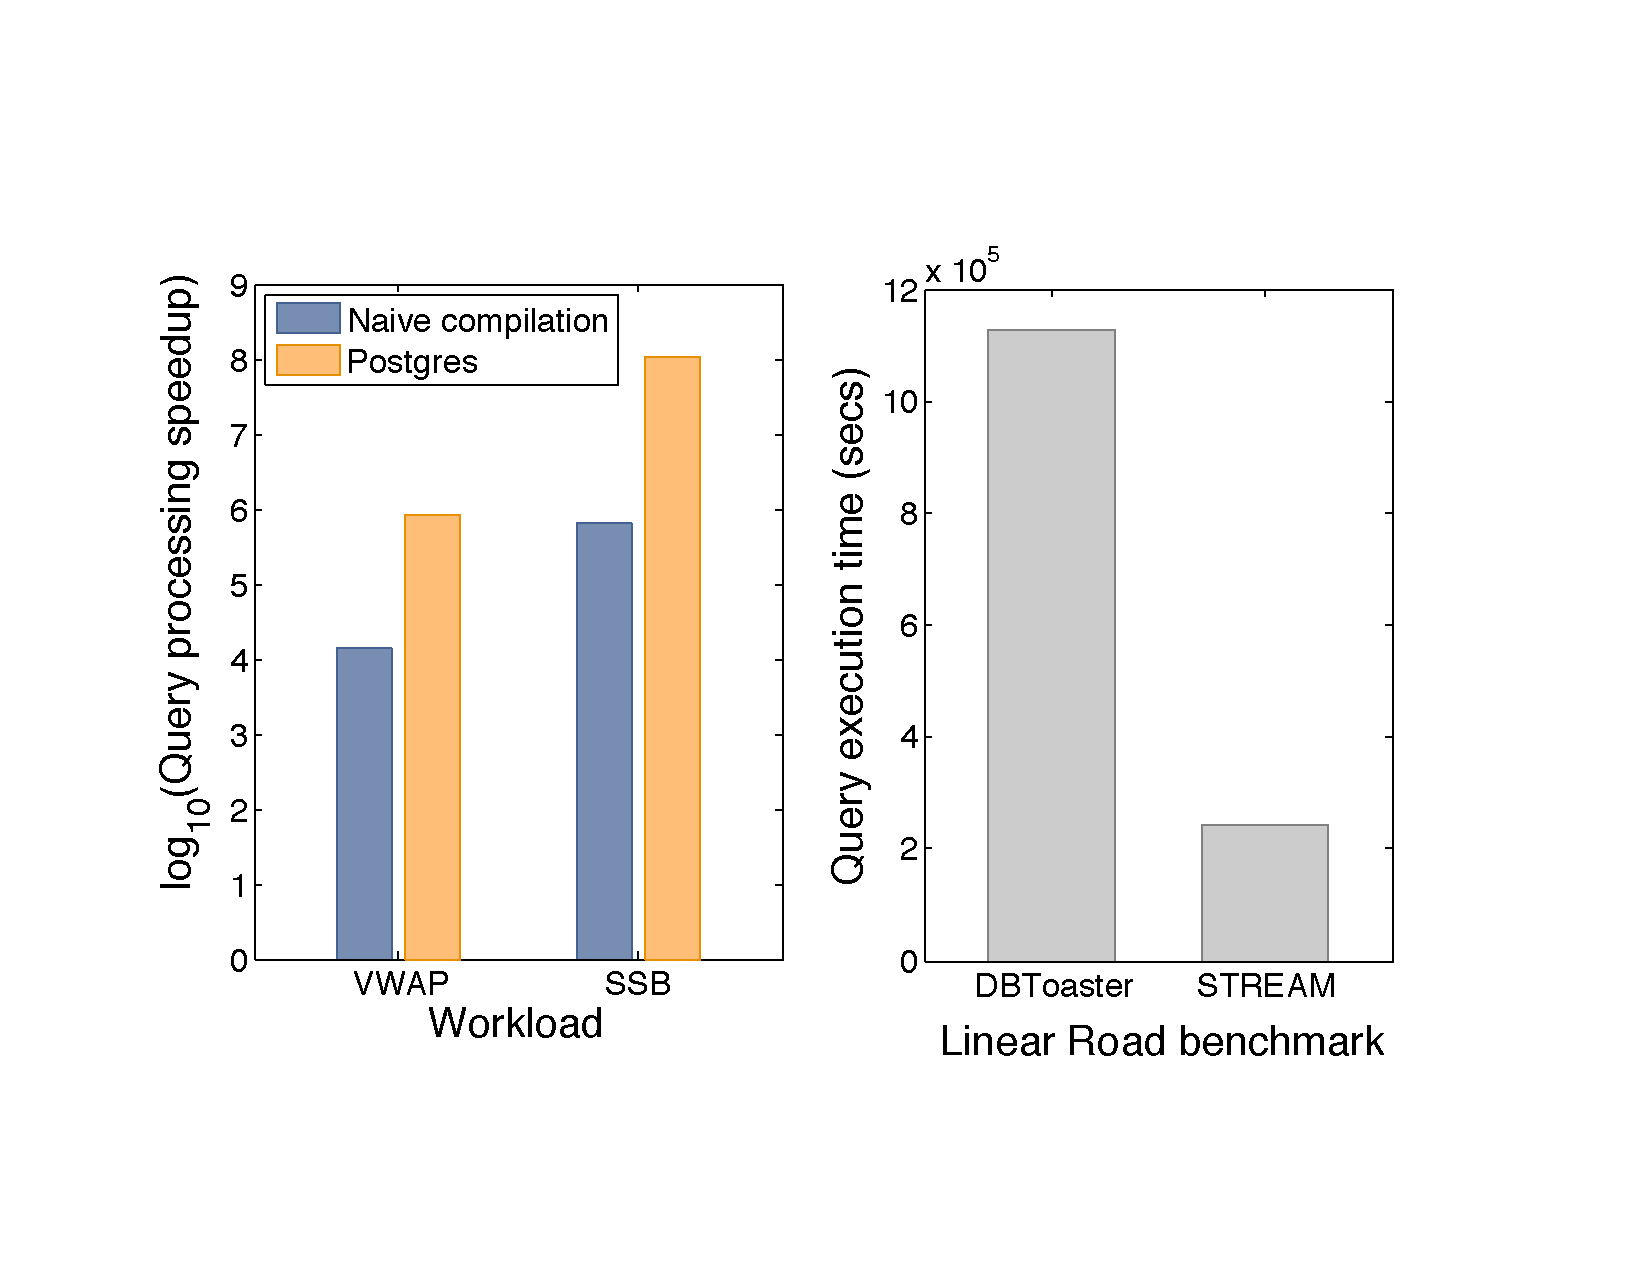
\includegraphics[scale=0.25]{../plots/toaster_comparison}
\end{center}
\caption{Query processing performance comparison of compiled query executors
generated by DBToaster and plan compilation, Postgres and STREAM}
\label{fig:dbtperf}
\end{figure}

\begin{figure}
\begin{center}
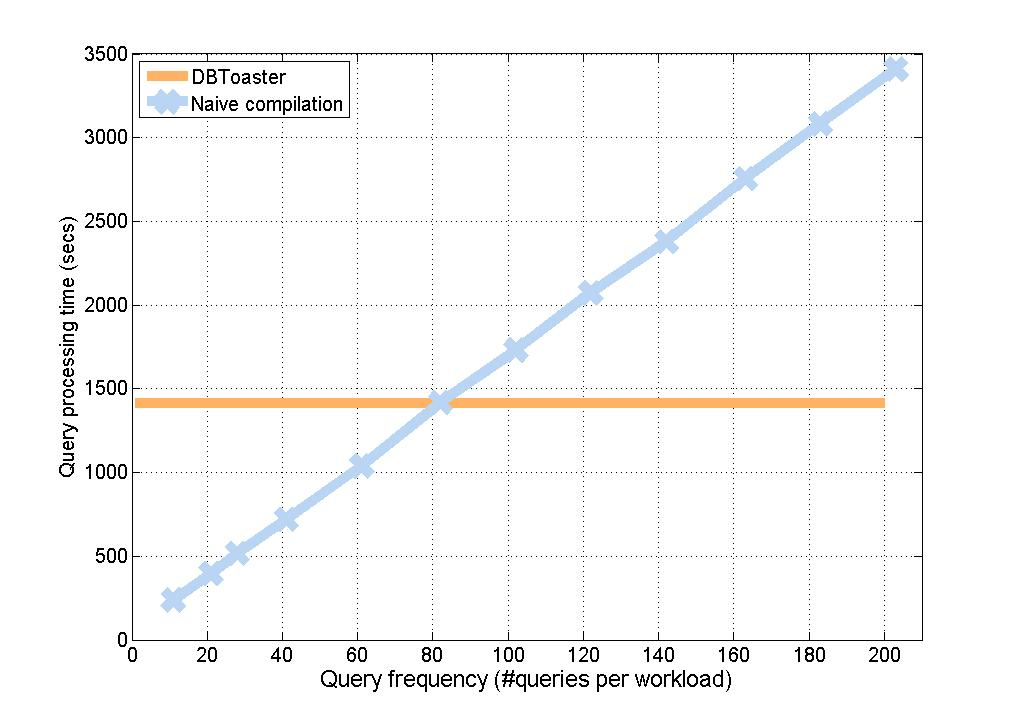
\includegraphics[scale=0.25]{../plots/vwap_query_freq_dn}
\end{center}
\caption{Query frequency limit for VWAP application, indicating the
query execution frequency beyond which DBToaster outperforms the naive query
plan compilation technique.}
\label{fig:vwap_query_freq}
\end{figure}

\begin{figure}
\begin{center}
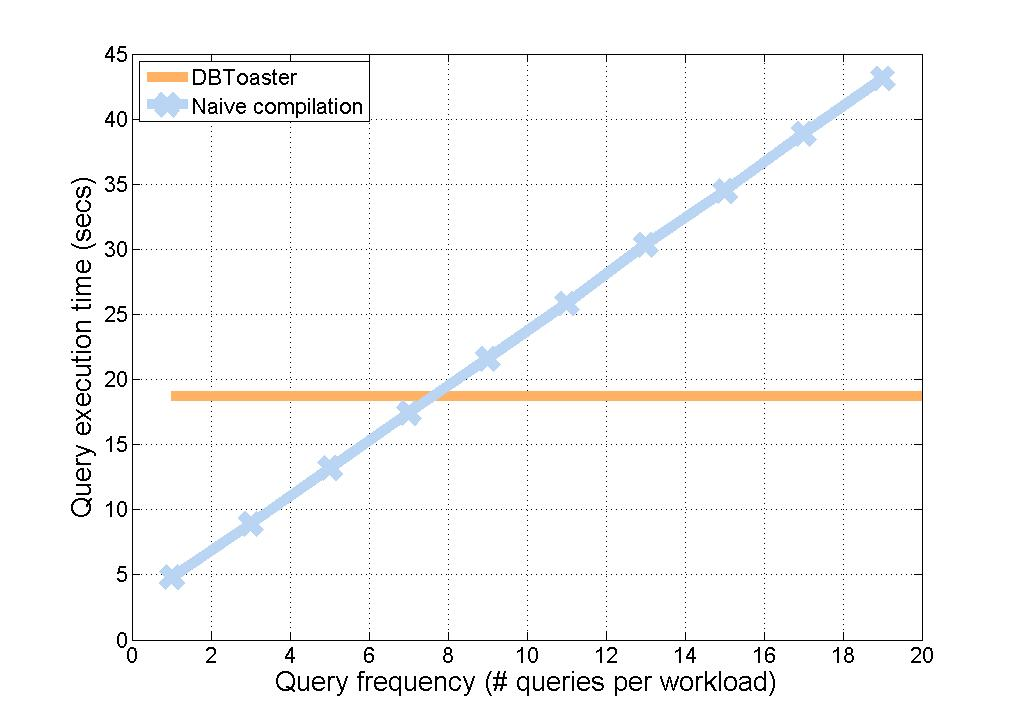
\includegraphics[scale=0.25]{../plots/ssb_query_freq_dn}
\end{center}
\caption{Query frequency limit for warehouse loading application, indicating the
query execution frequency beyond which DBToaster outperforms the naive query
plan compilation technique.}
\label{fig:ssb_query_freq}
\end{figure}

\subsection{Memory Analysis and Batch Execution}


\comment{
Dataset:

\begin{itemize}
  \item TotalView-ITCH dataset: 3 month's worth of MSFT order book messages
  taken from NASDAQ, (~2.2Gb dataset).
  \item Orderbook schema: day, time in us since beginning of day, order id,
  order type, share volume, bid/ask price
\end{itemize}

Queries:

\begin{verbatim}
select * from
  (select ax_bids.mmid, abs(
    sum(ax_bids.volume*
      (act_now.expected_price - ax_bids.price)) -
    sum(ax_asks.volume*
      (ax_asks.price - act_now.expected_price)))
    as ax_bias
  from
    (select mmid, price, volume from bids
       where mmid in axs) as ax_bids,
    (select mmid, price, volume from asks
       where mmid in axs) as ax_asks,
    (select expected_price
        from technical_indicator
        where entrance_condition)
    as act_now
  where ax_bids.mmid = ax_asks.mmid
  group by ax_bids.mmid) as sneaky_ax,
where ax_bias > 10000
\end{verbatim}

Figures:

\begin{enumerate}
  \item Takeaway experiment: end-to-end throughput comparison for a variety of
  insert/update/delete rates. Requires replay speed parameter in data loader.
  Comparison points include Postgres, naive compilation, simple version
  of \compiler, \compiler\ with lazy evaluation, \compiler\ with bulk insert
  mode at 2 or 3 different chunk sizes.

  \item Detail experiment: analyse effect of bulk loading operations compared to
  simple compiler, on a variety of queries, e.g. selectivities and keys.
  Dependent variables for plots: cache hit rates for locality analysis,
  throughput to understand pipelining effects. Is there anything lower lever we
  can do for pipelining?

  \item Detail experiment: selectivity experiment, comparing \compiler\ w/ lazy
  eval, and w/ bulk loading (separately) to next best, for a variety of
  join selectivities and keys.

  \item Detail experiment: space vs recomputation analysis, where we vary the
  maps we keep between extremes of maps from simple decomposition, to full base
  tables.

  \item Quality of compiled code, and compiler effect? e.g. speed provided with
  different -O flags?

\end{enumerate}
}